\documentclass{beamer}
\usetheme[titleformat=regular,sectiontitleformat=regular,frametitleformat=regular]{m}

\usepackage[brazil]{babel}
\usepackage[numberedbib]{apacite}
\usepackage[utf8]{inputenc}
\usepackage{mathabx}
\usepackage{tabularx}
\usepackage{lipsum}
\usepackage{multicol}

\newcommand\Fontvi{\fontsize{7}{7.2}\selectfont}


\title{Uma abordagem evolutiva ao problema de record linkage}
\date{\today}
\author{Acadêmico: Herberth Amaral \\
Orientador: Prof. Dr. Renê Rodrigues Veloso}
\institute{Programa de Pós-Graduação em Modelagem Computacional e Sistemas - UNIMONTES}
\begin{document}
  \maketitle

  \section{Problema}

  \begin{frame}{Problema}
      \begin{itemize}
          \item Instituições com diferentes softwares para diferentes problemas;
          \item Várias bases de dados;
          \item Registros duplicados entre bases de dados;
      \end{itemize}
  \end{frame}

  \begin{frame}{Exemplo de duplicação de registros em uma instituição de saúde}
      \begin{figure}
          \centering
          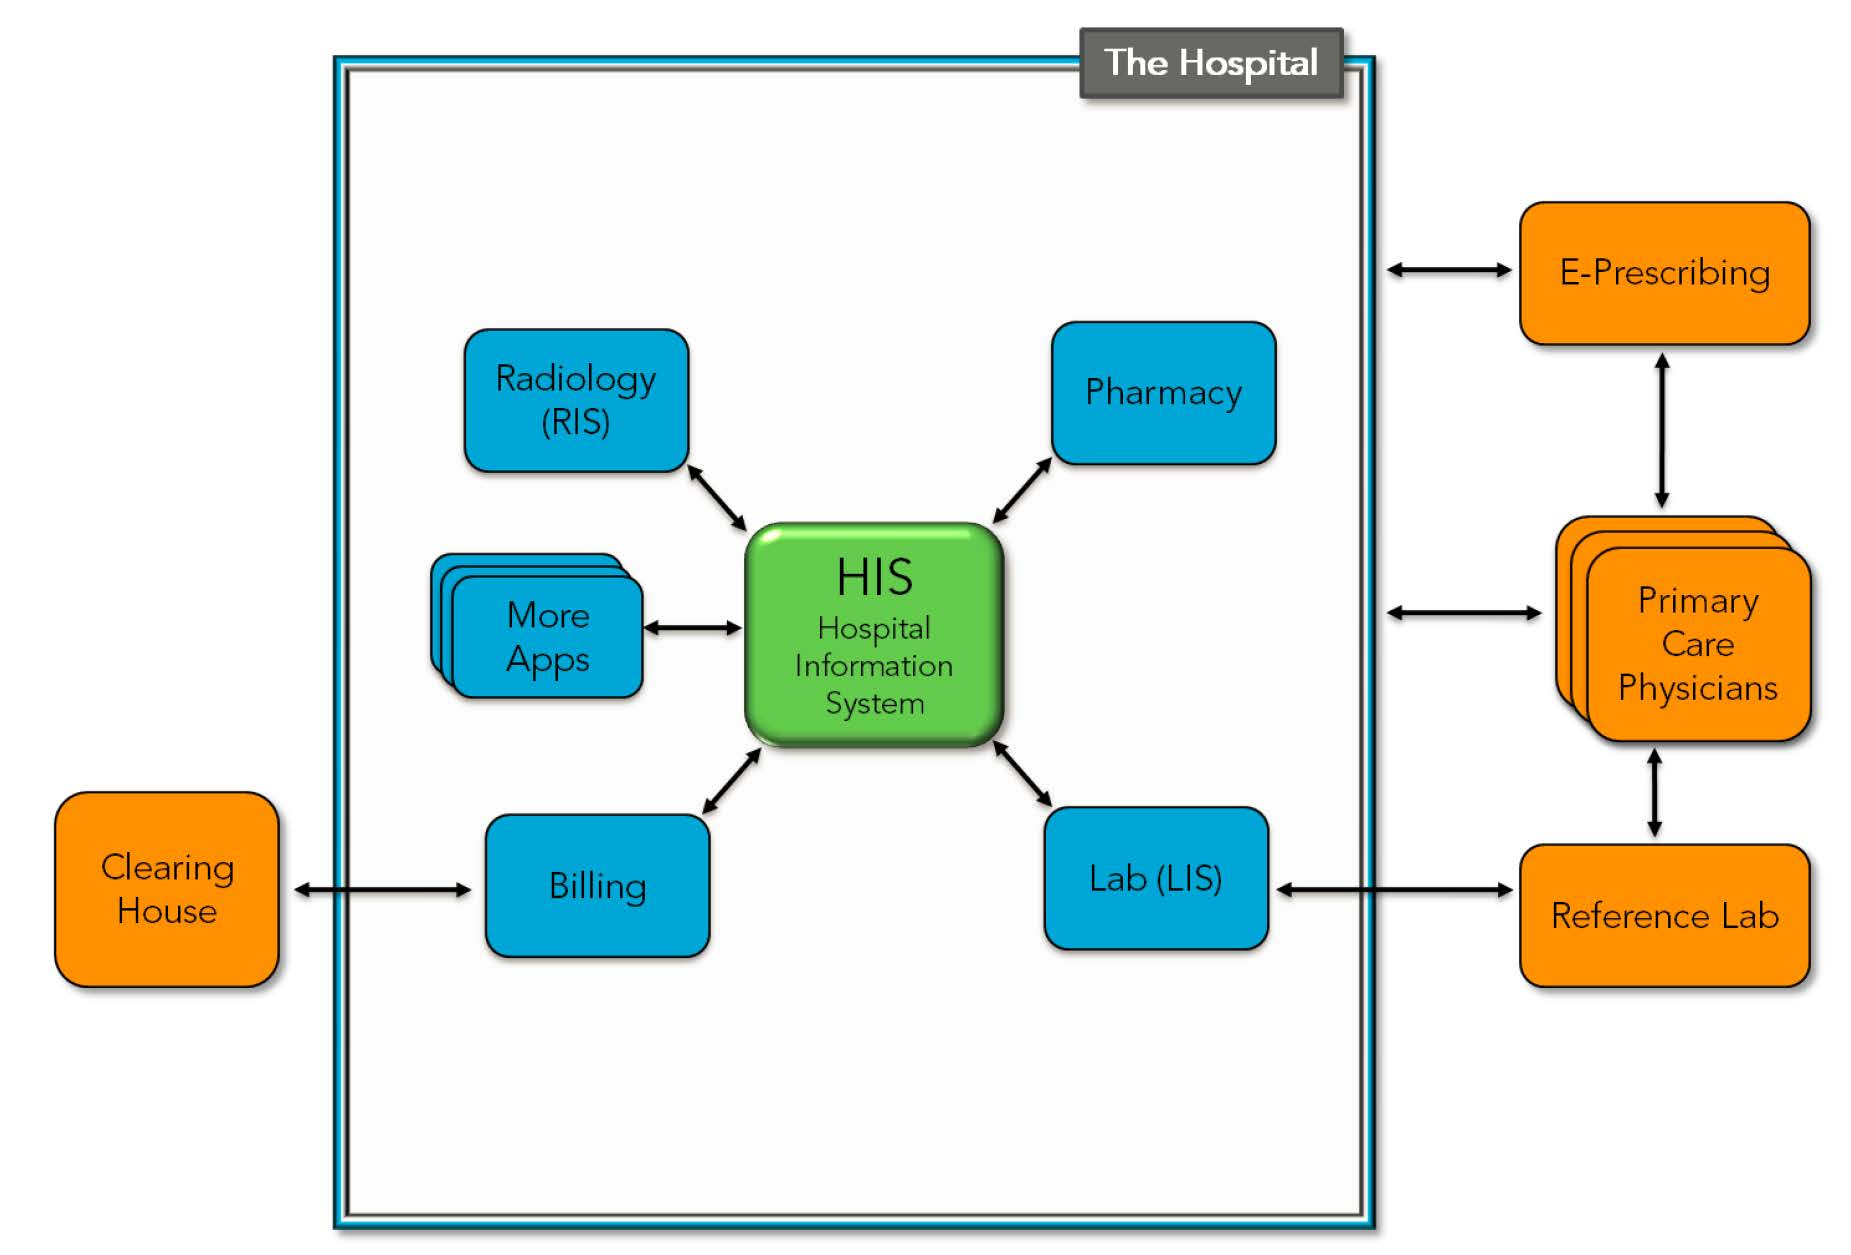
\includegraphics[width=1.0\textwidth]{hospital.jpg}
          \caption{Diferentes sistemas dentro de um hospital \cite{hospital}}
      \end{figure}
  \end{frame}

  \begin{frame}{Problemas com registros duplicados}
      Os principais problemas com registros duplicados/distribuídos em uma instituição de saúde são:

      \begin{itemize}
          \item Impossibilidade de unificação de prontuários de forma confiável;
          \item Dificuldades de comunicação entre diferentes setores (ex: farmácia e financeiro);
          \item Erros de diagnóstico;
          \item Falta de confiança em processos informatizados.
      \end{itemize}
  \end{frame}

  \section{Record linkage}

  \begin{frame}{Introdução à RL}
      \begin{itemize}
          \item \textit{Record linkage} (RL) é o processo de identificação de registros duplicados que representam a mesma entidade em um ou mais bases de dados \cite{survey};
          \item Permite a unificação de dados a partir de um ponto em comum (ex: paciente).
      \end{itemize}
  \end{frame}

  \begin{frame}{Processo de RL}
      \begin{figure}
          \centering
          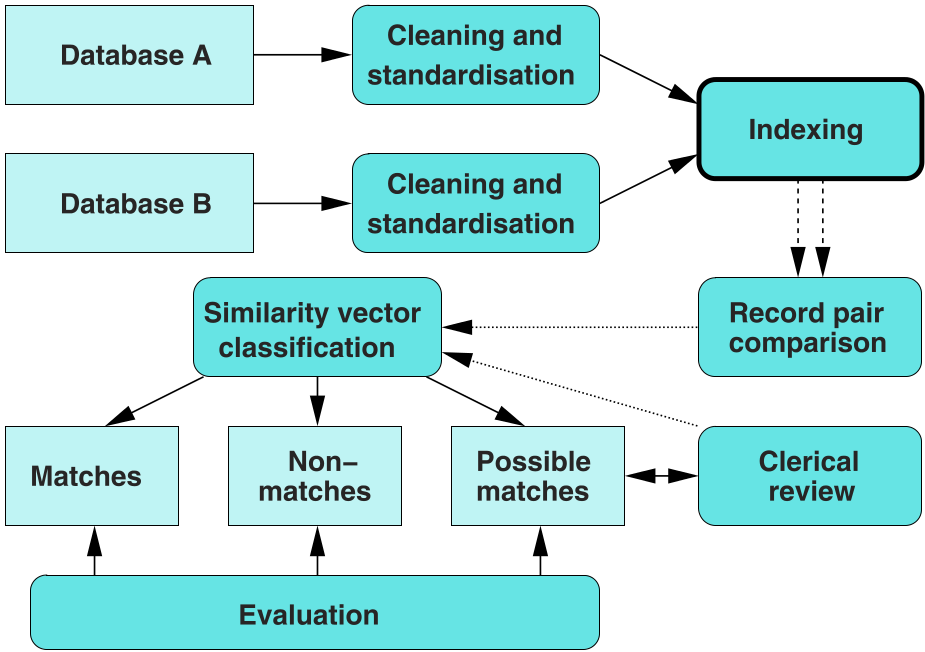
\includegraphics[width=0.9\textwidth]{rlprocess.png}
          \caption{Processo de record linkage \cite{survey}}
      \end{figure}
  \end{frame}

  \begin{frame}{Funções de similaridade para comparação de registros}
      \begin{table}
          \centering
          \caption{Algumas funções de similaridade \cite{survey}}
          \begin{tabularx}{\textwidth}{|l|X|}
              \hline
              Função                    & Observação \\ \hline
              Jaro                      & Principalmente para primeiros e últimos nomes. Retorna um valor no intervalo $[0,1]$ em que 0 é diferente e 1 é igual. \\ \hline
              Jaro-Winkler              & Baseado na Jaro. Dá mais pesos à prefixos. \\ \hline
              Levenshtein               & Número de edições entre duas strings. 0 significa que são iguais\\ \hline
              Similaridade de cosenos   & Intervalo $[-1, 1]$. Muito utilizado em busca em textos. \\ \hline
          \end{tabularx}
      \end{table}
  \end{frame}

  \begin{frame}{Breve exemplo}
      Considere dois bancos de dados de exemplo:
      \Fontvi
      \begin{multicols}{2}
          \begin{table}[]
              \centering
              \caption{Banco de dados A}
              \begin{tabular}{|l|l|l|l|}
                  \hline
                  ID & Nome  & Sobrenome & Nascimento \\ \hline
                  1  & Luís  & Silva     & 1990-05-01 \\
                  2  & Marco & Túlio     & 1978-03-14 \\ \hline
              \end{tabular}
          \end{table}
          \columnbreak
          \begin{table}[]
              \centering
              \caption{Banco de dados B}
              \begin{tabular}{|l|l|l|l|}
                  \hline
                  ID & Nome   & Sobrenome & Nascimento \\ \hline
                  1  & Luiz   & Silva     & 1990-01-05 \\
                  2  & Marcos & Tulio     & 1978-03-14 \\
                  3  & Pedro  & Ferreira  & 1989-10-21 \\ \hline
              \end{tabular}
          \end{table}
      \end{multicols}

      \textbf{Problema:} Como descobrir as duplicatas?
  \end{frame}

  \begin{frame}{Comparação campo-a-campo}
      \begin{table}[]
          \centering
          \caption{Comparação entre dois registros das bases de dados (depois da limpeza)}
          \label{tbl:comparacao}
          \begin{tabular}{|l|l|l|l|}
              \hline
              Função de comparação             & Nome & Sobrenome & Nascimento \\ \hline
              Jaro                             & luiz & silva     & 1990-05-01 \\
              Jaro                             & luis & silva     & 1990-01-05 \\ \hline
              \textbf{Resultado da comparação} & 0.83 & 1         & 0.96       \\ \hline
          \end{tabular}
      \end{table}

      Chamaremos de $E$ o vetor resultante da comparação.
  \end{frame}
  \begin{frame}{Regra de ligação (classificação)}
      Função que associa o vetor de comparação $E$ com a probabilidade do par de registros pertencerem a uma mesma entidade.

      \textbf{Exemplo:} \[
          F_s(E) = \begin{cases}
              1  &  \text{if }\dfrac{\sum \limits_{e \in E} e}{|E|} \geq 0.95 \\
              0  &  \text{otherwise} \\
          \end{cases}
      \]

      \textbf{Problema:} infelizmente, nem sempre a regra de ligação é tão simples.
  \end{frame}

  \section{Objetivos}
  \begin{frame}{Objetivo geral}
      Desenvolver um algoritmo de programação genética capaz de criar regras de
      ligação de registros com o intuito de aumentar a eficiência do processo de \textit{record linkage}.
  \end{frame}
  \begin{frame}{Objetivos específicos}
      \begin{itemize}
          \item Um algoritmo de programação genética eficiente do ponto de vista de melhores ajustes de regras de ligação;
          \item Adaptações dos operadores de programação genética capazes de permitir o uso de evolução diferencial;
          \item Extensões de algoritmos para comparação de pares de registros em meio a dados faltantes.
      \end{itemize}
  \end{frame}

  \section{Referência: A Genetic Programming Approach to Record Deduplication (Carvalho, 2012)}

  \begin{frame}{Modelagem de RL com GP - Linhas gerais}

      \textbf{Objetivo:} Evolução de uma função de similaridade $F_s: E \mapsto [0,1]$.

      \textbf{Parâmetros}: conjunto de \textit{evidências}, em que cada evidência $E$ é um par $(atributo, func. similaridade)$, exemplo:
      \begin{center}
      $E = \{(nome, Jaro), (sobrenome, Jaro), (endereco, Jaro)\}$.
      \end{center}

      \textbf{Exemplo de função de similaridade:}
      \begin{center}
          $F_s(E) = \dfrac{\sum \limits_{e \in E} e}{|E|}$
      \end{center}
  \end{frame}

  \begin{frame}{Função objetivo}
      A função de \textit{fitness} utilizada na evolução da árvore é o F1-score, assim definida:

      \begin{center}
          $P = \dfrac{V_p}{V_p+F_p}$ \\
          $R = \dfrac{V_p}{V_p+F_n}$ \\
          $F1 = 2*\dfrac{PR}{P+R}$ \\
      \end{center}
      Em que: $V_p$ são os verdadeiros-positivos, $F_p$ são os falsos-positivos e $F_n$ são os falsos-negativos.
  \end{frame}

  \begin{frame}{Experimentos}
      Os datasets utilizados foram:
      \begin{enumerate}
          \item \textbf{Cora bibliographic} - uma coleção de citações - 1295 instâncias. \textbf{Atributos}: \textit{author names, year, title, venue, pages} e \textit{other info}.
          \item \textbf{Restaurant dataset} - endereços de restaurantes -- 864 instâncias, sendo 112 duplicadas. \textbf{Atributos}: \textit{name, address, city} e \textit{specialty}.
          \item Datasets genéricos utilizando o SDG do FEBRL.
      \end{enumerate}
  \end{frame}

  \begin{frame}{Experimentos - evidência manualmente selecionadas}
      A imagem \ref{fig:tbl1} mostra os resultados dos testes executados.
      \begin{figure}
          \centering
          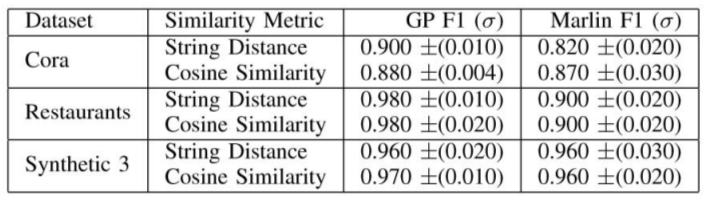
\includegraphics[width=0.75\textwidth]{resultados-manuais.png}
          \caption{Resultados da estratégia manual \cite{geneticrl}}
          \label{fig:tbl1}
      \end{figure}
  \end{frame}

  \begin{frame}{Discussão dos resultados}
      \begin{itemize}
          \item Uso de uma abordagem $O(n^2)$;
          \item Bases de dados pequenas (máximo de 1295 registros);
          \item Alto tempo de treinamento.
      \end{itemize}
  \end{frame}

  \section{Oportunidades de pesquisa}
  \begin{frame}{Oportunidades de pesquisa}
      \Fontvi
      \begin{itemize}
          \item Inserção de parâmetros de índice para diminuição do espaço de busca;
          \item Modelagem multi-objetivo do problema de record linkage;
          \item Adaptação da função Jaro-Winkler para o contexto local;
          \item Evolução diferencial para programação genética;
          \item Uso de técnicas de evolução gramatical \cite{grammatical-evolution} para o problema de record linkage;
          \item Modelagem do problema de record linkage para algoritmos genéticos.
      \end{itemize}
  \end{frame}

  \begin{frame}{Cronograma}
      \begin{figure}
          \centering
          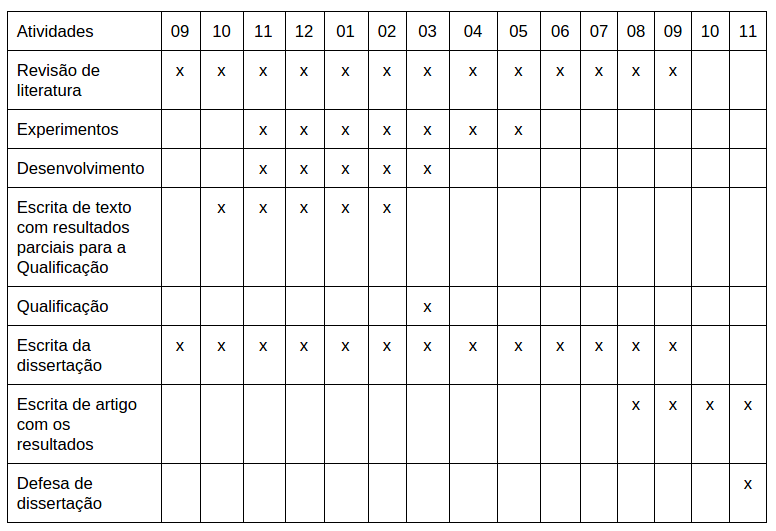
\includegraphics[width=0.9\textwidth]{cronograma.png}
      \end{figure}
  \end{frame}

  \section{Perguntas}
  \section{Muito obrigado!}
  \begin{frame}{Códigos}
      Os códigos dos experimentos feitos até agora estão disponibilizados em \url{https://github.com/herberthamaral/mestrado/tree/master/ProjetoDissertacao}.
  \end{frame}

  %\begin{frame}{Modelagem utilizando evolução diferencial}
  %    Abordagem similar à abordagem GP, mas com a seguinte função de similaridade:
  %    \begin{center}
  %        $F_s(E,W) = \sum\limits_{e \in E,w \in W} e*w ; |E| = |W|$
  %    \end{center}
  %\end{frame}


  \begin{frame}
      \bibliographystyle{apacite}
      \bibliography{apresentacao}
  \end{frame}
\end{document}
